\subsection{Кинематика вращательного движения: угловая скорость и угловое ускорение, их связь с линейной скоростью и ускорением}

При движении по окружности аналогом пройденного пути выступает угол $\varphi$, на который повернулось тело относительно оси вращения. 
Измеряется в радианах. 
$\vec\varphi$ направлен вверх при вращении против часовой стрелки (правило правого винта).

\begin{definition}
    Угловая скорость $[\omega, \frac{рад}{с}]$ — векторная величина, характеризующая быстроту и направление вращения материальной точки 
или абсолютно твердого тела относительно центра вращения.
\end{definition}

\begin{remark}
    Угловая скорость характеризует изменение угла поворота со временем.

    Угловая скорость — вектор, направление которого совпадает с осью вращения и определяется по правилу правого винта.

    В трёхмерном пространстве вектор угловой скорости по величине равен углу поворота точки вокруг центра вращения за единицу времени.
\end{remark}

\begin{definition}
    Мгновенная угловая скорость — предел, к которому стремится средняя угловая скорость при $\Delta t\to0$:
$$
\omega=\frac{d\varphi}{dt}
$$
\end{definition}

\begin{definition}
    Период обращения точки $[T, с]$ — время, за которое точка совершает один полный оборот.
    
    $$T=\frac{2\pi R}{\upsilon}=\frac{2\pi}{\omega}$$
\end{definition}

\begin{definition}
    Частота обращения точки $[\nu, с^{-1}]$ — величина, равная числу оборотов в единицу времени.

    $$
    \nu=\frac{1}{T}
    $$
\end{definition}

\begin{remark}
    Центростремительное ускорение $[a_ц]$:
    
    $$a_ц=\omega^2R=\frac{\upsilon^2}{R}=\frac{4\pi^2}{T^2}R=4\pi^2\nu^2R$$
\end{remark}

\begin{definition}
    Угловое ускорение $[\varepsilon, \frac{рад}{с^2}]$ — величина, характеризующая изменение угловой скорости с течением времени.
\end{definition}

\begin{definition}
    Мгновенное угловое ускорение — предел среднего ускорения при $\Delta t\to0$:

    $$\vec\varepsilon=\frac{d\vec\omega}{dt}=\frac{d^2\vec\varphi}{dt^2}$$
\end{definition}

\begin{wrapfigure}{l}{0.2\linewidth}
    \centering
    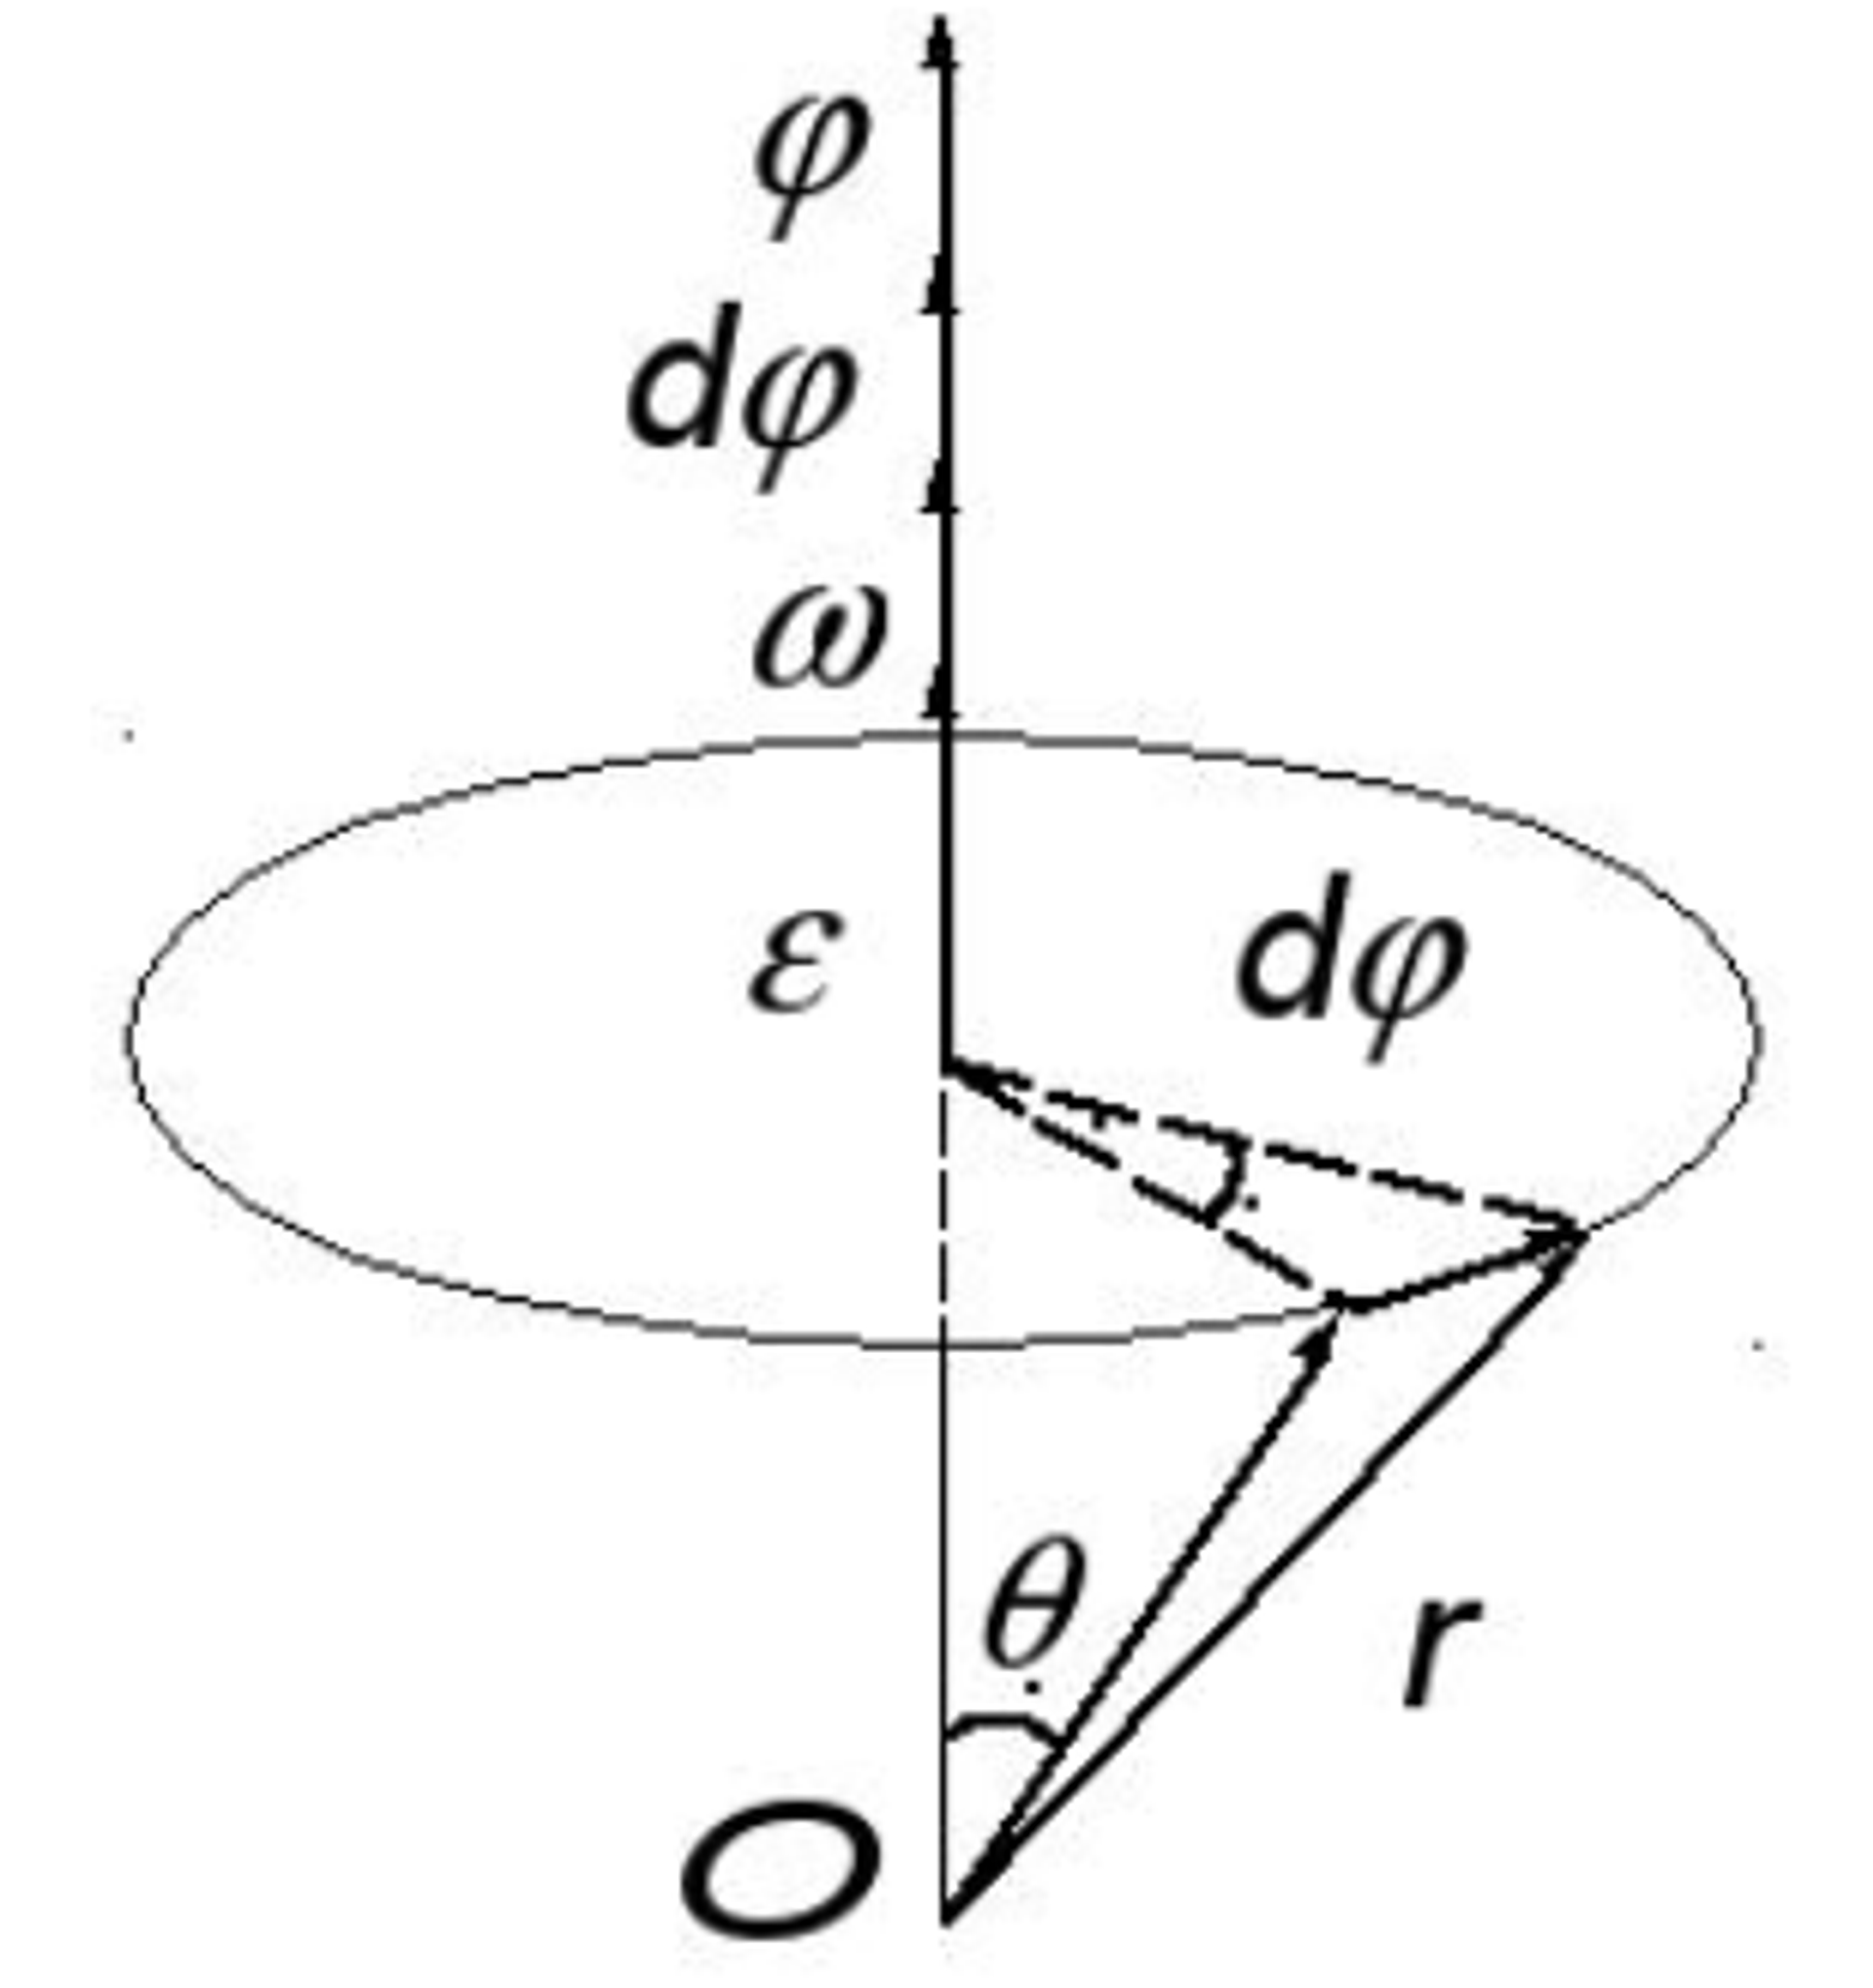
\includegraphics[width=\linewidth]{imgs/q2i1.png}
\end{wrapfigure}

Угол поворота $\varphi$.

Угловая скорость $\omega=\frac{d\varphi}{dt}$

Угловое ускорение $\varepsilon=\frac{d\omega}{dt}$

Если $|\vec\omega|\uparrow\ \Rightarrow\ \varepsilon\uparrow\uparrow\omega$,

Если $|\vec\omega|\downarrow\ \Rightarrow\ \varepsilon\downarrow\uparrow\omega$

Если $\varepsilon=const$ (равноускоренное движение), то:$\displaystyle\\ \omega(t)=\omega_0+\varepsilon\cdot t$, $\displaystyle\\\Delta\vec\varphi(t)=\vec\omega_0\cdot t+\frac{\varepsilon\cdot t^2}{2}$.

\begin{figure}[h]
    \centering
    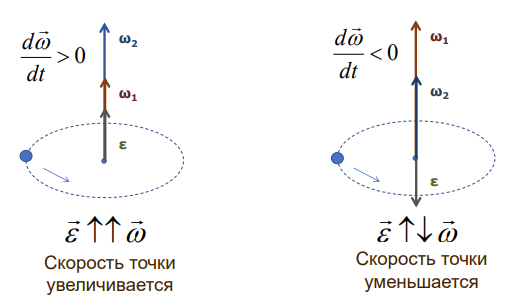
\includegraphics[width=0.5\linewidth]{imgs/q2i2.png}
\end{figure}


\begin{remark}
    Связь линейной скорости с угловой скоростью.

    $$
    \upsilon=\frac{2\pi R}{T}=2\pi R\nu \implies \upsilon=\omega R
    $$

    Соответственно, чем дальше расположена точка тела от оси вращения, тем больше её линейная скорость.
\end{remark}

\begin{remark}
    Связь между линейным и угловым ускорениями

    $a_n = \frac{v^2}{R} = \omega^2\cdot R$
    $a_\tau = \dot{v} = R \cdot \dot{\omega} = \varepsilon \cdot R$

    Полное ускорение $\vec{a} = \vec{a_\tau} + \vec{a_n}$

    $a = \sqrt{a_\tau^2 + a_n^2} = \sqrt{(\varepsilon R)^2 + (\omega^2 R)^2} = R\sqrt{\varepsilon^2+\omega^4}$
\end{remark}

\begin{figure}[h]
    \centering
    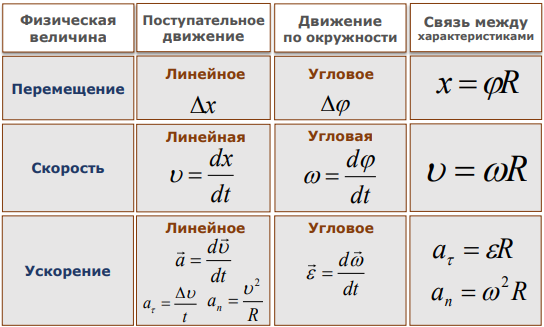
\includegraphics[width=0.5\linewidth]{imgs/q2i3.png}
    \caption{Аналогии между линейными и угловыми характеристиками движения}
\end{figure}

\begin{figure}[h]
    \centering
    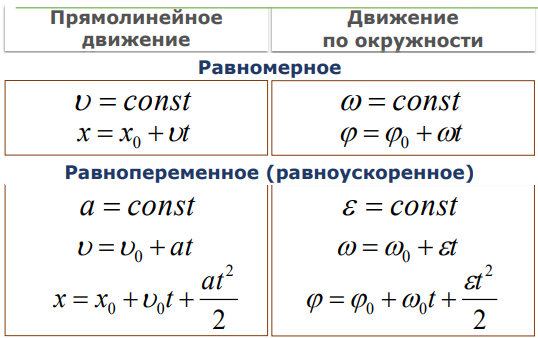
\includegraphics[width=0.5\linewidth]{imgs/q2i4.png}
    \caption{Аналогии между законами прямолинейного движения и движения по окружности}
\end{figure}